% tirlnx01 - Materiaal om het keuzevak Linux te geven 
% op de Hogeschool Rotterdam.
% Copyright (C) 2010 - 2011  Paul Sohier, Kevin van der Vlist
%
% This program is free software: you can redistribute it and/or modify
% it under the terms of the GNU General Public License as published by
% the Free Software Foundation, either version 3 of the License, or
% (at your option) any later version.
%
% This program is distributed in the hope that it will be useful,
% but WITHOUT ANY WARRANTY; without even the implied warranty of
% MERCHANTABILITY or FITNESS FOR A PARTICULAR PURPOSE.  See the
% GNU General Public License for more details.
%
% You should have received a copy of the GNU General Public License
% along with this program.  If not, see <http://www.gnu.org/licenses/>.
%
% Kevin van der Vlist - kevin@kevinvandervlist.nl
% Paul Sohier - paul@paulsohier.nl

\documentclass{beamer}

\mode<presentation>

\usepackage[dutch]{babel}
\usepackage{listings}
%\usepackage{beamerthemesplit}

\lstset{ %
  language=bash,                % choose the language of the code
  basicstyle=\footnotesize,       % the size of the fonts that are used for the code
  numbers=left,                   % where to put the line-numbers
  numberstyle=\footnotesize,      % the size of the fonts that are used for the line-numbers
  numbersep=5pt,                  % how far the line-numbers are from the code
  showspaces=false,               % show spaces adding particular underscores
  showstringspaces=false,         % underline spaces within strings
  showtabs=false,                 % show tabs within strings adding particular underscores
  frame=lr,	                % adds left and right lines
  tabsize=2,	                % sets default tabsize to 2 spaces
  captionpos=b,                   % sets the caption-position to bottom
  breaklines=true,                % sets automatic line breaking
  breakatwhitespace=false,        % sets if automatic breaks should only happen at whitespace
%  escapeinside={\%*}{*)},         % if you want to add a comment within your code
  morekeywords={*,...}            % if you want to add more keywords to the set
}

\usetheme{Berlin}
\useinnertheme{rounded}
\usecolortheme{rose}
\setbeamertemplate{navigation symbols}{} 

\title{Keuzevak Linux - Week 2}
\author{Paul Sohier \and Kevin van der Vlist}
\institute{Versie $1.0$}
\date{\today}

\begin{document}

\begin{frame}
  \titlepage
\end{frame} 

\begin{frame}
  \frametitle{Inhoud}
  \tableofcontents
\end{frame}

\section{Gebruikers en groepen}

\begin{frame}
  \frametitle{Gebruikers en groepen - algemeen}
  \begin{itemize}
  \item<1-> multi user omgeving
  \item<2-> 1 user : $n$ groepen
  \item<3-> speciaal: \texttt{root}
  \end{itemize}
\end{frame}

\begin{frame}[fragile]
  \frametitle{Gebruikers en groepen - /etc/passwd}
  \begin{lstlisting}
lp:x:4:7:lp:/var/spool/lpd:/bin/false
  \end{lstlisting}
  \begin{itemize}
  \item<2-> bevat alle gebruikers informatie
  \item<3-> wachtwoord is speciaal
  \end{itemize}
\end{frame}

\begin{frame}[fragile]
  \frametitle{Gebruikers en groepen - /etc/shadow}
% user:pass:lastpwchange:minpwage:maxpwage:pwwarnperiod
  \begin{lstlisting}
lp:*:9797:0:::::
kevin:$1$8f4unajknfi488afaklj40ud:14950:0:99999:7:::
paul:!:14963:0:99999:7:::
  \end{lstlisting}
  \begin{itemize}
  \item<2-> lp: geen login
  \item<3-> kevin: wachtwoord hash
  \item<4-> paul: geblokkeerd
  \item<5-> standaard slackware hash:
    \begin{lstlisting}
root@slackbak:/home/kevin# grep ENCRYPT_METHOD /etc/login.defs
ENCRYPT_METHOD MD5
    \end{lstlisting}
  \end{itemize}
\end{frame}

\begin{frame}[fragile]
  \frametitle{Gebruikers en groepen - /etc/group}
  \begin{lstlisting}
adm:x:4:root,adm,daemon
tty:x:5:
  \end{lstlisting}
  \begin{itemize}
  \item<2-> adm heeft drie leden
  \item<3-> tty geen
  \end{itemize}
\end{frame}

\begin{frame}[fragile]
  \frametitle{Gebruikers en groepen - /etc/\{passwd,shadow,group\}}
  \begin{lstlisting}
root@slackbak:/etc# ls -l {shadow,passwd,group}
-rw-r--r-- 1 root root    685 Dec  8 10:47 group
-rw-r--r-- 1 root root   1148 Jan 14 14:21 passwd
-rw-r----- 1 root shadow  711 Jan 14 14:21 shadow
  \end{lstlisting}
  \begin{itemize}
  \item<2-> user, group en other
  \item<3-> \texttt{/etc/shadow} : rechten
  \item<4-> reden? Veiligheid
  \end{itemize}
\end{frame}

\section{Runlevels}

\begin{frame}
  \frametitle{Runlevels - algemeen}
  \begin{itemize}
  \item<1-> status van het systeem
  \item<2-> duiden taken aan
  \item<3-> slackware:\\
    \begin{tabular}[t]{ll}
      \hline
      runlevel & taken\\
      \hline
      0 & halt\\
      1 & single user mode\\
      2,3 & multi user mode\\
      4 & 3 + X11\\
      6 & reboot\\
    \end{tabular}
  \end{itemize}
\end{frame}

\begin{frame}[fragile]
  \frametitle{Runlevels - /etc/inittab}
  \begin{itemize}
    \item<1-> runlevels worden door \texttt{init} aangestuurd
    \item<2-> configuratiefile voor \texttt{init}
    \item<3-> definitie default runlevel:
      \begin{lstlisting}
root@slackbak:/etc# grep initdefault inittab
id:3:initdefault:
      \end{lstlisting}
  \end{itemize}
\end{frame}

\section{Manual pages}

\begin{frame}
  \frametitle{Manual pages - algemeen}
  \begin{itemize}
  \item<1-> handleidingen
  \item<2-> \texttt{man man}
  \item<3-> see also shadow(5) : \texttt{man 5 shadow}
  \end{itemize}
\end{frame}

\begin{frame}
  \frametitle{Manual pages - beschrijving}
  \begin{itemize}
  \item<1-> \texttt{NAME}: naam en korte omschrijving
  \item<2-> \texttt{SYNOPSIS}: syntax
  \item<3-> \texttt{DESCRIPTION}: uitgebreide beschrijving
  \item<4-> \texttt{OPTIONS}: alle opties
  \item<5-> \texttt{SEE ALSO}: verwijzing relevante documentatie
  \end{itemize}
\end{frame}

\begin{frame}[fragile]
  \frametitle{Manual pages - voorbeeld}
  \begin{lstlisting}
NAME
       manexample - Een voorbeeld manual
SYNOPSIS
       manexample  [-f  file]  [-d]  [-D]  [--warnings[=warnings]]  [-R  encoding]  [-L  locale] page
DESCRIPTION
       Dit is een voorbeeld van een manual. Er staat hier een uitgebreide beschrijving.
EXAMPLES
       manexample manpage
           Laat de voorbeeld manual van manpage zien.
OPTIONS
       -L locale, --locale=locale
              Start met een bepaald locale
SEE ALSO
       mandb(8), manpath(1)
  \end{lstlisting}
\end{frame}

\begin{frame}
  \frametitle{Manual pages - navigatie}
  \begin{itemize}
  \item<1-> regel vooruit: \texttt{enter}
  \item<1-> pagina vooruit: \texttt{spatie} of \texttt{f}
  \item<1-> pagina terug: \texttt{b}
  \item<1-> vooruit zoeken: \texttt{/zoekterm}
  \item<1-> teruguit zoeken: \texttt{?zoekterm}
  \item<2-> meer informatie: \texttt{man less}
  \end{itemize}
\end{frame}

\section{Filesystem}

\begin{frame}
  \frametitle{Filesystem - informatie}
  \begin{itemize}
  \item[1.] \texttt{cd} - \textbf{C}hange \textbf{D}irectory
  \item[2.] \texttt{cp} - \textbf{C}o\textbf{p}y
  \item[3.] \texttt{ls} - \textbf{L}i\textbf{s}t
  \item[4.] \texttt{mkdir} - \textbf{M}a\textbf{k}e \textbf{Dir}ectory
  \item[5.] \texttt{pwd} - \textbf{P}rint \textbf{W}orking \textbf{D}irectory
  \item[6.] \texttt{rm} - \textbf{R}e\textbf{m}ove
  \item[7.] \texttt{rmdir} - \textbf{R}e\textbf{m}ove \textbf{Dir}ectory
  \item[8.] \texttt{df} - \textbf{D}isk \textbf{F}ree
  \end{itemize}
\end{frame}

\begin{frame}
  \frametitle{Filesystem - layout}
  \setlength{\unitlength}{1mm}
  \begin{center}
    \begin{picture}(90, 50)
      \thicklines
      % lvl 0
      % Root node
      \put(30,45){\circle{15}}
      \put(30,45){\makebox(0,1){\texttt{/}}}
      % Arrows
      \put(30,38){\vector(-3,-2){10}}
      \put(30,38){\vector(3,-2){10}}

      % lvl 1
      % usr
      \put(15,25){\circle{15}}
      \put(15,25){\makebox(0,1){\texttt{usr}}}
      % Arrows
      \put(15,18){\vector(-3,-2){10}}
      % home
      \put(45,25){\circle{15}}
      \put(45,25){\makebox(0,1){\texttt{home}}}
      % Arrows
      \put(45,18){\vector(-3,-2){10}}
      \put(45,18){\vector(0,-2){5}}
      \put(45,18){\vector(3,-2){10}}

      % lvl 2
      % usr/bin
      \put(0,5){\circle{15}}
      \put(0,5){\makebox(0,1){\texttt{bin}}}
      % home/femke
      \put(30,5){\circle{15}}
      \put(30,5){\makebox(0,1){\texttt{femke}}}
      % home/kevin
      \put(45,5){\circle{15}}
      \put(45,5){\makebox(0,1){\texttt{kevin}}}
      % home/paul
      \put(60,5){\circle{15}}
      \put(60,5){\makebox(0,1){\texttt{paul}}}
    \end{picture}
  \end{center}
\end{frame}

\begin{frame}
  \frametitle{Filesystem - mounten}
  \begin{itemize}
  \item<1-> systemcall \texttt{mount}
  \item<2-> \texttt{mount -t ntfs-3g /dev/sdb1 /media/usbstick}
  \item<3-> systemcall \texttt{umount}
  \item<4-> \texttt{umount /media/usbstick}
  \item<5-> speciaal: \texttt{mount -a}
  \end{itemize}
\end{frame}

\begin{frame}[fragile]
  \frametitle{Filesystem - /etc/fstab}
  \begin{lstlisting}
kevin@slackbak:~$ cat /etc/fstab
/dev/sda1  /          ext4 defaults        1 1
/dev/sda2  /home      xfs  defaults        1 2
/dev/cdrom /mnt/cdrom auto noauto,owner,ro 0 0
  \end{lstlisting}%$
% dump, fsck order
\end{frame}

\begin{frame}
  \frametitle{Filesystem - recovery}
  \begin{itemize}
  \item<1-> \texttt{fsck}
  \item<2-> detecteren van fouten
  \item<3-> repareren van fouten
  \item<4-> \texttt{fsck /dev/sda1}
  \item<5-> \texttt{tune2fs}, \texttt{xfs\_check}
  \end{itemize}
\end{frame}

\section{Editors}

\begin{frame}
  \frametitle{Editors - nano/pico}
  \begin{itemize}
  \item<1-> simpel
  \item<2-> vergelijkbaar met kladblok
  \end{itemize}
\end{frame}

\begin{frame}
  \frametitle{Editors - vi(m)}
  \begin{itemize}
  \item<1-> geavanceerder
  \end{itemize}
  \begin{figure}[H]
    \begin{center}
      
\includegraphics[scale=0.2]{images/vimschoonmaak}
    \end{center}
    \caption{vim editor}
    \label{fig:editor_vim}
  \end{figure}
\end{frame}

\begin{frame}
  \frametitle{Editors - emacs}
  \begin{itemize}
  \item<1-> meest geavanceerd
  \end{itemize}
  \begin{figure}[H]
    \begin{center}
      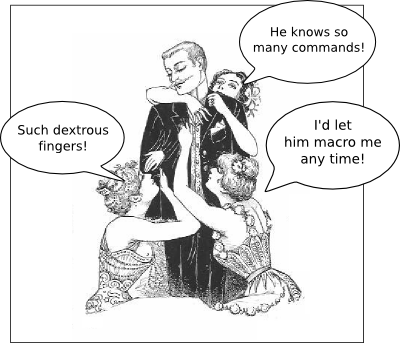
\includegraphics[scale=0.4]{images/emacsmanwomen}
    \end{center}
    \caption{emacs editor}
    \label{fig:editor_emacs}
  \end{figure}
\end{frame}

\end{document}

